\documentclass[10pt,border=2pt]{standalone}
\usepackage[T1]{fontenc}
\usepackage{lmodern}
\usepackage{pgfplots}
\pgfplotsset{compat=1.18}
\definecolor{localblue}{HTML}{0072B2}
\definecolor{localpurple}{HTML}{AA4499}
\definecolor{localorange}{HTML}{D97700}
\definecolor{localgreen}{HTML}{009E73}
\begin{document}
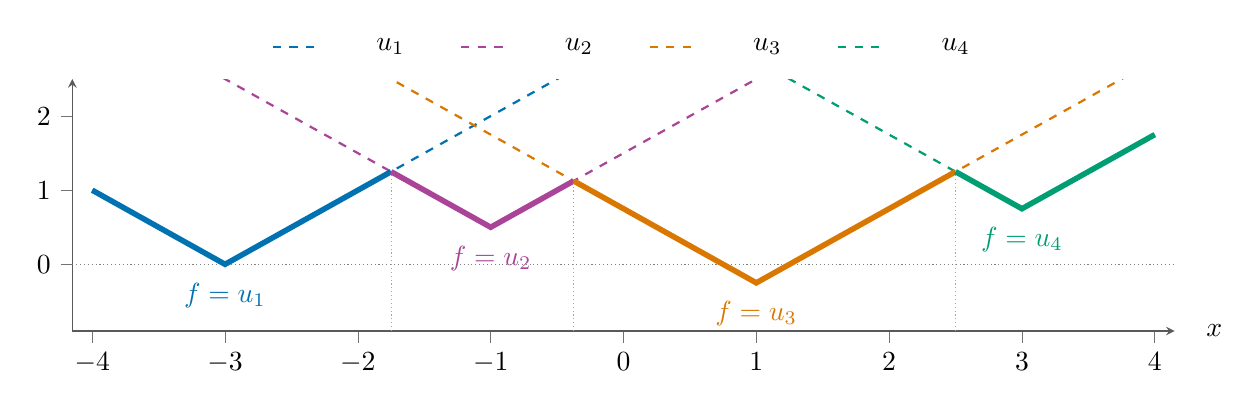
\begin{tikzpicture}
\begin{axis}[
  scale only axis,width=14cm,height=3.2cm,
  xmin=-4.15,xmax=4.15,ymin=-0.9,ymax=2.5,
  xtick={-4,-3,-2,-1,0,1,2,3,4},ytick={0,1,2},
  axis lines=left,axis line style={black!65},
  tick align=outside,tick style={black!55},
  xlabel={$x$},xlabel style={at={(axis description cs:1.02,0)},anchor=west},
  label style={font=\normalsize},tick label style={font=\normalsize},
  legend style={at={(0.5,1.05)},anchor=south,draw=none,font=\normalsize,
    legend columns=4,column sep=18pt},
  clip=true,
]
\addplot[black!50,densely dotted,thin,forget plot] coordinates {(-4.15,0) (4.15,0)};
\addplot[black!35,densely dotted,thin,forget plot] coordinates {(-1.75,-0.9) (-1.75,1.25)};
\addplot[black!35,densely dotted,thin,forget plot] coordinates {(-0.375,-0.9) (-0.375,1.125)};
\addplot[black!35,densely dotted,thin,forget plot] coordinates {(2.5,-0.9) (2.5,1.25)};
\addplot[localblue,thick,dashed] coordinates {(-4,1) (-3,0) (4,7)};
\addlegendentry{$u_1$}
\addplot[localpurple,thick,dashed] coordinates {(-4,3.5) (-1,0.5) (4,5.5)};
\addlegendentry{$u_2$}
\addplot[localorange,thick,dashed] coordinates {(-4,4.75) (1,-0.25) (4,2.75)};
\addlegendentry{$u_3$}
\addplot[localgreen,thick,dashed] coordinates {(-4,7.75) (3,0.75) (4,1.75)};
\addlegendentry{$u_4$}
\addplot[localblue,line width=2pt,forget plot] coordinates {(-4,1) (-3,0) (-1.75,1.25)};
\addplot[localpurple,line width=2pt,forget plot] coordinates {(-1.75,1.25) (-1,0.5) (-0.375,1.125)};
\addplot[localorange,line width=2pt,forget plot] coordinates {(-0.375,1.125) (1,-0.25) (2.5,1.25)};
\addplot[localgreen,line width=2pt,forget plot] coordinates {(2.5,1.25) (3,0.75) (4,1.75)};
\node[anchor=north,localblue] at (axis cs:-3,-0.12) {$f=u_1$};
\node[anchor=north,localpurple] at (axis cs:-1,0.38) {$f=u_2$};
\node[anchor=north,localorange] at (axis cs:1,-0.37) {$f=u_3$};
\node[anchor=north,localgreen] at (axis cs:3,0.63) {$f=u_4$};
\end{axis}
\end{tikzpicture}
\end{document}
